\documentclass[11pt]{book}

% Use the ETAMU physics style package
\usepackage{../../shared/styles/etamu-physics}

% Document metadata
\title{Level 1 Physics\\Instructor Manual}
\author{ETAMU Physics Department}
\date{\today}

\begin{document}

\frontmatter
\maketitle

\tableofcontents
\listoffigures

\chapter{Preface}

Welcome to the Level 1 Physics Instructor Manual. This manual provides comprehensive coverage of introductory physics topics with detailed solutions, teaching notes, and extensive LaTeX examples for creating professional physics documents.

\section{How to Use This Manual}

This manual is designed to:
\begin{itemize}
    \item Provide complete solutions to all problems
    \item Demonstrate best practices for typesetting physics content
    \item Include LaTeX tutorials throughout for common physics elements
    \item Serve as a template for creating additional course materials
\end{itemize}

\section{LaTeX Resources}

Throughout this manual, you'll find tutorial boxes that explain how to create various elements in LaTeX. These are designed to help you modify and extend the course materials effectively.

\mainmatter

\chapter{Mechanics}

\section{Kinematics}

\begin{tutorialbox}[title=Typesetting Physics Equations]
To create physics equations, use the \texttt{physics} package commands:
\begin{verbatim}
\[ \vect{v} = \dv{\vect{r}}{t} \]
\[ \vect{a} = \dv{\vect{v}}{t} = \dv[2]{\vect{r}}{t} \]
\end{verbatim}
This produces:
\[ \vect{v} = \dv{\vect{r}}{t} \]
\[ \vect{a} = \dv{\vect{v}}{t} = \dv[2]{\vect{r}}{t} \]
\end{tutorialbox}

The fundamental kinematic equations describe motion with constant acceleration:

\begin{align}
    \vect{v} &= \vect{v}_0 + \vect{a}t \label{eq:velocity} \\
    \vect{r} &= \vect{r}_0 + \vect{v}_0 t + \frac{1}{2}\vect{a}t^2 \label{eq:position} \\
    v^2 &= v_0^2 + 2a\Delta x \label{eq:velocity-squared}
\end{align}

\begin{problembox}[title=Example Problem 1.1]
A car accelerates from rest at \SI{2.0}{\meter\per\second\squared} for \SI{5.0}{\second}. Find:
\begin{enumerate}[label=(\alph*)]
    \item The final velocity
    \item The distance traveled
\end{enumerate}
\end{problembox}

\textbf{Solution:}

Given: $v_0 = \SI{0}{\meter\per\second}$, $a = \SI{2.0}{\meter\per\second\squared}$, $t = \SI{5.0}{\second}$

\begin{tutorialbox}[title=Using SI Units]
Always use the \texttt{siunitx} package for units:
\begin{verbatim}
\SI{2.0}{\meter\per\second\squared}
\SI{5.0}{\second}
\end{verbatim}
This ensures proper spacing and formatting.
\end{tutorialbox}

(a) Using \cref{eq:velocity}:
\begin{align}
    v &= v_0 + at \\
    &= \SI{0}{\meter\per\second} + (\SI{2.0}{\meter\per\second\squared})(\SI{5.0}{\second}) \\
    &= \SI{10.0}{\meter\per\second}
\end{align}

(b) Using \cref{eq:position}:
\begin{align}
    x &= x_0 + v_0 t + \frac{1}{2}at^2 \\
    &= \SI{0}{\meter} + (\SI{0}{\meter\per\second})(\SI{5.0}{\second}) + \frac{1}{2}(\SI{2.0}{\meter\per\second\squared})(\SI{5.0}{\second})^2 \\
    &= \SI{25.0}{\meter}
\end{align}

\section{Forces and Newton's Laws}

\begin{tutorialbox}[title=Creating Force Diagrams with TikZ]
Use TikZ to create clear force diagrams:
\begin{verbatim}
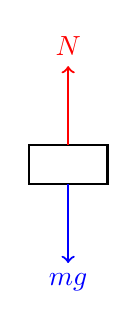
\begin{tikzpicture}
  \draw[thick] (0,0) rectangle (1,0.5);
  \draw[->,red,thick] (0.5,0.5) -- (0.5,1.5) node[above] {$\vect{N}$};
  \draw[->,blue,thick] (0.5,0) -- (0.5,-1) node[below] {$m\vect{g}$};
\end{tikzpicture}
\end{verbatim}
\end{tutorialbox}

Newton's three laws form the foundation of classical mechanics:

\begin{enumerate}
    \item \textbf{First Law (Inertia):} An object at rest stays at rest, and an object in motion stays in motion at constant velocity, unless acted upon by a net external force.
    
    \item \textbf{Second Law:} The acceleration of an object is directly proportional to the net force acting on it and inversely proportional to its mass:
    \[ \sum \vect{F} = m\vect{a} \]
    
    \item \textbf{Third Law:} For every action, there is an equal and opposite reaction.
\end{enumerate}

\chapter{Energy and Work}

The work-energy theorem states that the work done on an object equals its change in kinetic energy:

\[ W = \Delta KE = \frac{1}{2}mv_f^2 - \frac{1}{2}mv_i^2 \]

\begin{tutorialbox}[title=Creating Energy Diagrams]
Use PGFPlots for energy graphs:
\begin{verbatim}
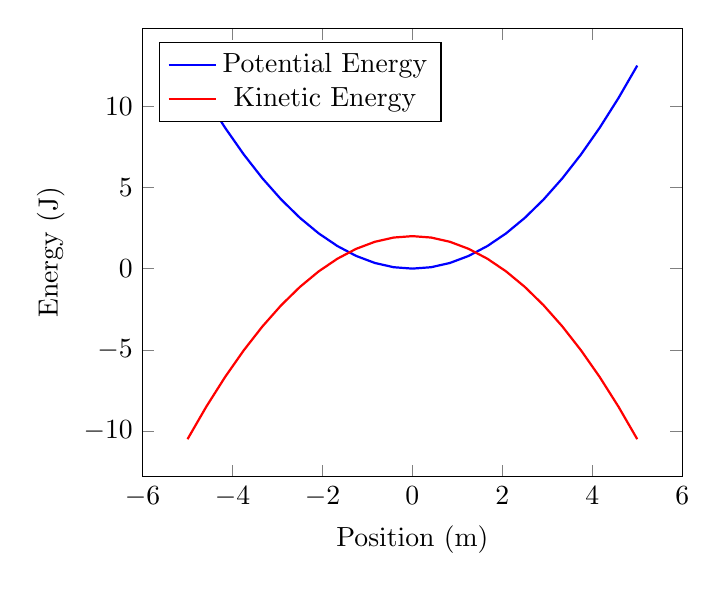
\begin{tikzpicture}
\begin{axis}[
    xlabel={Position (m)},
    ylabel={Energy (J)},
    legend pos=north west
]
\addplot[blue,thick] {x^2/2};
\addlegendentry{Potential Energy}
\addplot[red,thick] {2-x^2/2};
\addlegendentry{Kinetic Energy}
\end{axis}
\end{tikzpicture}
\end{verbatim}
\end{tutorialbox}

\backmatter

\appendix

\chapter{LaTeX Quick Reference}

\section{Common Physics Symbols}
\begin{tabular}{ll}
    \toprule
    Symbol & LaTeX Command \\
    \midrule
    $\vect{F}$ & \texttt{\textbackslash vect\{F\}} \\
    $\uvect{r}$ & \texttt{\textbackslash uvect\{r\}} \\
    $\dv{x}{t}$ & \texttt{\textbackslash dv\{x\}\{t\}} \\
    $\pdv{f}{x}$ & \texttt{\textbackslash pdv\{f\}\{x\}} \\
    $\SI{9.8}{\meter\per\second\squared}$ & \texttt{\textbackslash SI\{9.8\}\{\textbackslash meter\textbackslash per\textbackslash second\textbackslash squared\}} \\
    \bottomrule
\end{tabular}

\section{Useful Packages}
\begin{itemize}
    \item \texttt{physics} - Physics notation and operators
    \item \texttt{siunitx} - SI units and number formatting
    \item \texttt{tikz} - Creating diagrams and figures
    \item \texttt{pgfplots} - Plotting graphs and data
    \item \texttt{circuitikz} - Circuit diagrams
\end{itemize}

\end{document}